%%%%(c) COPYRIGHT NOTICE%FOLDUP
%%%%(c)
%%%%(c)  This file is a portion of the source for the textbook
%%%%(c)
%%%%(c)    Numerical Methods Course Notes,
%%%%(c)    Copyright 2004-2010 by Steven E. Pav
%%%%(c)
%%%%(c)  See the file COPYING.txt for copying conditions
%%%%(c)
%%%%(c)%UNFOLD

%%throat clearing%FOLDUP
\typeout{-- odes.tex}
\typeout{-- N� 2004-2010 Steven E. Pav}
%UNFOLD

%%local commands%FOLDUP
\providecommand{\RK}[0]{Runge-Kutta\xspace}
\providecommand{\RKM}[0]{\RK Method\xspace}
\providecommand{\EM}[0]{Euler's Method\xspace}
\providecommand{\BEM}[0]{Backwards Euler's Method\xspace}
%UNFOLD

\chapter{Ordinary Differential Equations}\label{chap:odes}

Ordinary Differential Equations, or ODEs, are used in approximating some
physical systems.  Some classical uses include simulation of the growth of
populations and trajectory of a particle.  They are usually easier to solve or
approximate than the more general Partial Differential Equations, PDEs, which
can contain partial derivatives.

Much of the background material of this chapter should be familiar to the
student of calculus.  We will focus more on the approximation of solutions,
than on analytical solutions.  For more background on ODEs, see any of the
standard texts, \eg \cite{Sjcalc5}.

%%%%%%%%%%%%%%%%%%%%%%%%%%%%%%%%%%%%%%%%%%%%%%%
\section{Elementary Methods}%FOLDUP
\label{sec:odeelem}
\depson{sec:taylors}{sec:odeelem}

A one-dimensional ODE is posed as follows: find some function $x(t)$ such that
\begin{equation}
\left\{ \begin{array}{l} \dbyd{x(t)}{t} = f\Parens{t,x(t)},\\x(a) = c.\end{array}\right.
\label{eqn:onedode}
\end{equation}
In calculus classes, you probably studied the case where $f\Parens{t,x(t)}$ is
independent of its second variable.  For example the ODE given by 
\[\left\{ \begin{array}{l} \dbyd{x(t)}{t} = t^2 - t,\\x(a) = c.\end{array}\right.\]
has solution $x(t) = \oneby{3}t^3 - \oneby{2}t^2 + K,$ where $K$ is chosen
such that $x(a) = c.$

A more general case is when $f(t,x)$ is separable, that is
$f(t,x) = g(t)h(x)$ for some functions $g,h$.  You may recall that the solution
to such a separable ODE usually involved the following equation:
\[\int \frac{\dx}{h(x)} = \int g(t)\dx[t]\]

Finding an analytic solution can be considerably more difficult in the general
case, thus we turn to approximation schemes.

%%%%%%%%%%%%%%%%%%%%%%%%%%%%%%%%%%%%%%%%%%%%%%%
\subsection{Integration and `Stepping'}%FOLDUP

\index{ODE!stepping}%
We attempt to solve the ODE by integrating both sides.  That is
\begin{align}
\dbyd{x(t)}{t} &= f\Parens{t,x(t)}, \quad \text{yields}\nonumber\\
\int_t^{t+h} \dx  &= \int_t^{t+h} f\Parens{r,x(r)}\dx[r], \quad
\text{thus}\nonumber\\
x(t+h) &= x(t) + \int_t^{t+h} f\Parens{r,x(r)}\dx[r].\label{eqn:intgltodiffl}
\end{align}
If we can approximate the integral then we have a way of `stepping' from $t$ to
$t+h$, \ie if we have a good approximate of $x(t)$ we can approximate $x(t+h)$.  
Note that this means that all the work we have put into approximating integrals
can be used to approximate the solution of ODEs.

Using stepping schemes we can approximate $x(t_{final})$ given $x(t_{initial})$
by taking a number of steps.  For simplicity we usually use the same step size,
$h$, for each step, though nothing precludes us from varying the step size.

If we apply the left-hand rectangle rule for approximating integrals to
\eqnref{intgltodiffl}, we get

\begin{empheq}[box=\widefbox]{equation}%FOLDUP
x(t+h) \approx x(t) + h f(t,x(t)).
\label{eqn:eulerdef}\end{empheq}
%UNFOLD
This is called \emph{\EM{}.}\index{Euler's Method}
Note this is essentially the same as the ``forward difference'' approximation
we made to the derivative, \eqnref{fwddiff}.

Trapezoid rule gives
\begin{align*}
x(t+h) &\approx x(t) + \half[h] \Bracks{f(t,x(t)) + f(t+h,x(t+h))}.
\end{align*}
But we cannot evaluate this exactly, since $x(t+h)$ appears on both sides of
the equation.  And it is embedded on the right hand side. Bummer.  But if we
could approximate it, say by using \EM, maybe the formula would
work.  This is the idea behind the \RKM (see
\secref{rkmethods}).

%UNFOLD

%%%%%%%%%%%%%%%%%%%%%%%%%%%%%%%%%%%%%%%%%%%%%%%
\subsection{Taylor's Series Methods}%FOLDUP

\index{Taylor's Series Method}%
We see that our more accurate integral approximations will be useless since
they require information we do not know, \ie evaluations of $f(t,x)$ for yet unknown
$x$ values.  Thus we fall back on Taylor's Theorem (\bkthmref{taylors}).  We
can also view this as using integral approximations where all information comes
from the left-hand endpoint. 

By Taylor's theorem, if $x$ has at least $m+1$ continuous
derivatives on the interval in question, we can write
\[x(t+h) = x(t) + h x'(t) + \oneby{2} h^2 x''(t) + \ldots + \oneby{m!} h^m
x^{(m)}(t) + \oneby{(m+1)!} h^{m+1} x^{(m+1)}(\tau),\]
where $\tau$ is between $t$ and $t+h.$  Since $\tau$ is essentially unknown,
our best calculable approximation to this expression is
\[x(t+h) \approx x(t) + h x'(t) + \oneby{2} h^2 x''(t) + \ldots + \oneby{m!} h^m
x^{(m)}(t).\]
This approximate solution to the ODE is called a 
\emph{Taylor's series method of order $m.$}  We also say that this
approximation is a \emph{truncation} of the Taylor's series.  The difference
between the actual value of $x(t+h),$ and this approximation is called the
\emph{truncation error.}
The truncation error exists independently from any error in computing the
approximation, called roundoff error.  We discuss this more in
\subsecref{odeerrors}.

%Again we will use the idea of `stepping.'  $h$ is the step width.
%UNFOLD

%%%%%%%%%%%%%%%%%%%%%%%%%%%%%%%%%%%%%%%%%%%%%%%
\subsection{\EM}%FOLDUP

\index{Euler's Method}%
When $m=1$ we recover \EM:
\[x(t+h) = x(t) + hx'(t) = x(t) + hf(t,x(t)).\]

\begin{bkexample}\label{bkex:eultothex}%FOLDUP
Consider the ODE
\[\left\{ \begin{array}{l} \dbyd{x(t)}{t} = x,\\x(0) = 1.\end{array}\right.\]
The actual solution is $x(t) = \exp{t}.$  \EM will underestimate
$x(t)$ because the curvature of the actual $x(t)$ is positive, and thus the
function is always above its linearization.  In \figref{eulerep}, we see that 
eventually the \EM approximation is very poor. 
%
%\figref{eulerep}%FOLDUP
\begin{figure}[htb!]
\centering
	\psfrag{approx}[Br][r][0.8]{Euler approximation}
	\psfrag{actual}[Br][r][0.8]{Actual}
	\includegraphics[height=0.80\columnwidth,angle=270,clip=]{eulerep.eps}
\caption{\EM applied to approximate $x' = x,\,x(0)=1.$  Each step
proceeds on the linearization of the curve, and is thus an underestimate, as
the actual solution, $x(t) = \exp{t}$ has positive curvature.  Here step size
$h=0.3$ is used.}\label{fig:eulerep}
\end{figure}%UNFOLD
\end{bkexample}
%UNFOLD
%UNFOLD

%%%%%%%%%%%%%%%%%%%%%%%%%%%%%%%%%%%%%%%%%%%%%%%
\subsection{Higher Order Methods}%FOLDUP

\index{ODE!higher order methods}%
Higher order methods are derived by taking more terms of the Taylor's series
expansion.  Note however, that they will require information about the
higher derivatives of $x(t),$ and thus may not be appropriate for the case
where $f(t,x)$ is given as a ``black box'' function.

\begin{bkexprob}%FOLDUP
Derive the Taylor's series method for $m=3$ for the ODE
\[\left\{ \begin{array}{l} \dbyd{x(t)}{t} = x + \exp{x},\\x(0) = 1.\end{array}\right.\]
\begin{bksolution}
By simple calculus:
\begin{align*}
x'(t) &= x + \exp{x}\\
x''(t) &= x' + \exp{x} x' 
%= x'\Parens{1 + \exp{x}} = \Parens{x+\exp{x}}\Parens{1 + \exp{x}}
\\
x'''(t) &= x''\Parens{1+\exp{x}} + x' \exp{x} x' 
%= x'\Parens{1+\exp{x}}^2 + \exp{x} \Parens{x'}^2
\end{align*}
We can then write our step like a program:
\begin{align*}
x'(t) &\gets x(t) + \exp{x(t)}\\
x''(t) &\gets x'(t) \Parens{1+\exp{x(t)}}\\
x'''(t) &\gets x''(t) \Parens{1+\exp{x(t)}} + \Parens{x'(t)}^2 \exp{x(t)}\\
x(t+h) &\approx x(t) + hx'(t) + \oneby{2}h^2 x''(t) + \oneby{6}h^3 x'''(t)
% &= x(t) + h\Parens{x(t) + \exp{x(t)}} 
% + \frac{h^2}{2} \Parens{x(t)+\exp{x(t)}}\Parens{1 + \exp{x(t)}} 
% + \frac{h^3}{6} \Bracks{\Parens{x(t)+\exp{x(t)}}^2\exp{x(t)} +
% \Parens{x(t)+\exp{x(t)}}\Parens{1+\exp{x(t)}}^2}
\end{align*}
\end{bksolution}
\end{bkexprob}
%UNFOLD
%UNFOLD

%%%%%%%%%%%%%%%%%%%%%%%%%%%%%%%%%%%%%%%%%%%%%%%
\subsection{Errors}\label{subsec:odeerrors}%FOLDUP

\index{ODE!errors}\index{error!truncation}\index{error!roundoff}%
There are two types of errors: truncation and roundoff.
Truncation error is the error of truncating the Taylor's series after the
\kth{m} term.  You can see that the truncation error is \bigo{h^{m+1}}.
Roundoff error occurs because of the limited precision of
computer arithmetic.

While it is possible these two kinds of error could cancel each other, given
our pessimistic worldview, we usually assume they are additive.  
We also expect some tradeoff between these two errors as $h$ varies.  As $h$ is
made smaller, the truncation error presumably decreases, while the
roundoff error increases.  This results in an optimal $h$-value for a given
method.  See \figref{fakerror}.  Unfortunately, the optimal $h$-value will
usually depend on the given ODE and the approximation method.  For an ODE with
unknown solution, \emph{it is generally impossible to predict the optimal
$h$.} We have already observed this kind of behaviour, when analyzing
approximate derivatives--\cf \bkexpref{hdip}.

%\figref{fakerror}%FOLDUP
\begin{figure}[htb!]
\centering
	\psfrag{trunc(x)}[Br][r][0.8]{truncation}
	\psfrag{rndff(x)}[Br][r][0.8]{roundoff}
	\psfrag{error(x)}[Br][r][0.8]{total error}
	\includegraphics[width=0.75\columnwidth,angle=270,clip=]{fakerror.eps}
\caption{The truncation, roundoff, and total error for a fictional ODE and
approximation method are shown.   The total error is apparently minimized for
an $h$ value of approximately 0.0002.  Note that the truncation
error appears to be \bigo{h}, thus the approximation could be \EM.  In reality,
we expect the roundoff error to be more ``bumpy,'' as seen in \figref{hdip}.}\label{fig:fakerror}
\end{figure}%UNFOLD

Both of these kinds of error can accumulate:  Since we step from $x(t)$ to
$x(t+h),$ an error in the value of $x(t)$ can cause a greater error in the
value of $x(t+h).$  It turns out that for some ODEs and some methods, this does
not happen.  This leads to the topic of stability.
%UNFOLD

%%%%%%%%%%%%%%%%%%%%%%%%%%%%%%%%%%%%%%%%%%%%%%%
\subsection{Stability}\label{subsec:odestability}%FOLDUP

\index{ODE!stability}%
Suppose you had an exact method of solving an ODE, but had the wrong data.
That is, you were trying to solve
\[\left\{ \begin{array}{l} \dbyd{x(t)}{t} = f\Parens{t,x(t)},\\x(a) = c,\end{array}\right.\]
but instead fed the wrong data into the computer, which then solved exactly the
ODE
\[\left\{ \begin{array}{l} \dbyd{x(t)}{t} = f\Parens{t,x(t)},\\x(a) =
c+\epsilon.\end{array}\right.\]
This solution can diverge from the correct one because of the different
starting conditions.  We illustrate this with the usual example.

\begin{bkexample}\label{bkex:eposneg}
Consider the ODE
\[\dbyd{x(t)}{t} = x.\]
This has solution $x(t) = x(0)\exp{t}.$
The curves for different starting conditions diverge, as in \figref{epos}.

However, if we instead consider the ODE
\[\dbyd{x(t)}{t} = -x,\]
which has solution $x(t) = x(0)\exp{-t},$ we see that differences in the
initial conditions become immaterial, as in \figref{eneg}.

Thus the latter ODE exhibits stability: roundoff and truncation errors accrued
at a given step will become irrelevant as more steps are taken.  
The former ODE exhibits the opposite behavior--accrued errors will be amplified.

%\figref{eposneg}%FOLDUP
\begin{figure}[htbp!]
\centering
%\subfigure[$(1+\epsilon)\exp{t}$]{
\subfloat[$(1+\epsilon)\exp{t}$]{
	\psfrag{epos(0.5,x)}[Br][r][0.7]{$\epsilon = -0.5$}
	\psfrag{epos(0.75,x)}[Br][r][0.7]{$\epsilon = -0.25$}
	\psfrag{epos(1.0,x)}[Br][r][0.7]{$\epsilon = 0$}
	\psfrag{epos(1.25,x)}[Br][r][0.7]{$\epsilon = 0.25$}
	\psfrag{epos(1.5,x)}[Br][r][0.7]{$\epsilon = 0.5$}
	\label{fig:epos}
	\includegraphics[height=0.76\columnwidth,angle=270,clip=]{epos.eps}}\\
%\subfigure[$(1+\epsilon)\exp{-t}$]{
\subfloat[$(1+\epsilon)\exp{-t}$]{
	\psfrag{eneg(0.5,x)}[Br][r][0.7]{$\epsilon = -0.5$}
	\psfrag{eneg(0.75,x)}[Br][r][0.7]{$\epsilon = -0.25$}
	\psfrag{eneg(1.0,x)}[Br][r][0.7]{$\epsilon = 0$}
	\psfrag{eneg(1.25,x)}[Br][r][0.7]{$\epsilon = 0.25$}
	\psfrag{eneg(1.5,x)}[Br][r][0.7]{$\epsilon = 0.5$}
	\label{fig:eneg}
	\includegraphics[height=0.76\columnwidth,angle=270,clip=]{eneg.eps}}
\caption{Exponential functions with different starting conditions:
in (a), the functions $(1+\epsilon)\exp{t}$ are shown, while in (b),
$(1+\epsilon)\exp{-t}$ are shown.  The latter exhibits stability, while the
former exhibits instability.}\label{fig:eposneg}
\end{figure}%UNFOLD
\end{bkexample}

It turns out there is a simple test for stability.  If $f_x >
\delta$ for some positive $\delta,$ then the ODE is instable;  if $f_x < -
\delta$ for a positive $\delta,$ the equation is stable.  Some ODEs fall
through this test, however.

We can prove this without too much pain.  Define $x(t,s)$ to be the solution to 
\[\left\{ \begin{array}{l} \dbyd{x(t)}{t} = f\Parens{t,x(t)},\\x(a) = s,\end{array}\right.\]
for $t \ge a.$

Then instability means that
\[\lim_{t\to\infty} \abs{\prby{}{\px[s]} x(t,s)} = \infty.\]
Think about this in terms of the curves for our simple example $x' = x.$

If we take the derivative of the ODE we get
\begin{align*}
\prbypr{}{t} x(t,s) &= f(t,x(t,s)),\\
\prbypr{}{s} \prbypr{}{t} x(t,s) &= \prbypr{}{s} f(t,x(t,s)),\quad \text{\ie}\\
\prbypr{}{s} \prbypr{}{t} x(t,s) &= f_t(t,x(t)) \prbypr{t}{s} + f_x(t,x(t,s)) \prbypr{x(t,s)}{s}.
\end{align*}
By the independence of $t,s$ the first part of the RHS is zero, so
\begin{align*}
\prbypr{}{s} \prbypr{}{t} x(t,s) &= f_x(t,x(t,s)) \prbypr{x(t,s)}{s}.
\end{align*}
We use continuity of $x$ to switch the orders of differentiation:
\begin{align*}
\prbypr{}{t} \prbypr{}{s} x(t,s) &= f_x(t,x(t,s)) \prbypr{}{s}x(t,s).
\end{align*}
Defining $u(t) = \prbypr{}{s}x(t,s),$ and $q(t) = f_x(t,x(t,s)),$ we have
\begin{align*}
\prbypr{}{t} u(t) &= q(t) u(t).
\end{align*}
The solution is $u(t) = c \exp{Q(t)},$ where
\begin{align*}
Q(t) &= \int_a^t q(r) \dx[r].
\end{align*}
If $q(r) = f_x(r,x(r,s)) \ge \delta > 0,$ then $\lim Q(t) = \infty,$ and so
$\lim u(t) = \infty.$  But note that $u(t) = \prbypr{}{s} x(t,s),$ and thus we
have instability.

Similarly if $q(r) \le - \delta < 0,$ then $\lim Q(t) = -\infty,$ and so
$\lim u(t) = 0,$  giving stability.

%UNFOLD

%%%%%%%%%%%%%%%%%%%%%%%%%%%%%%%%%%%%%%%%%%%%%%%
\subsection{\BEM}\label{subsec:backwardsem}%FOLDUP

\index{Backwards Euler's Method}%

\EM is the most basic numerical technique for solving ODEs.  However, it may
suffer from instability, which may make the method inappropriate or
impractical.  However, it can be recast into a method which may have superior
stability at the cost of limited applicability.  

This method, the so-called \BEM, is a stepping method: given a
reasonable approximation to $x(t),$ it calculates an approximation to $x(t+h).$
As usual, Taylor's Theorem is the starting point.   Letting $t_f = t + h,$
Taylor's Theorem states that
\[
x(t_f - h) = x(t_f) + (-h) x'(t_f) + \frac{(-h)^2}{2} x''(t_f) + \ldots,
\]
for an analytic function.  Assuming that $x$ has two continuous derivatives on
the interval in question, the second order term is truncated to give
\begin{align*}
x(t) = x(t + h - h) = 
x(t_f - h) &\approx  x(t_f) + (-h) x'(t_f)\\
\text{and so,}\qquad\,x(t + h) &\approx x(t) + h x'(t + h)\\
\end{align*}

The complication with applying this method is that $x'(t+h)$ may not be
computable if $x(t+h)$ is not known, thus cannot be used to calculate an 
approximation for $x(t+h).$  Since this approximation may contain $x(t+h)$ on
both sides, we call this method an \emph{implicit method}.  In contrast, \EM,
and the \RK methods in the following section are \emph{explicit methods}: they
can be used to directly compute an approximate step.  We make this clear by
examples.

\begin{bkexample}%FOLDUP
Consider the ODE
\[\left\{ \begin{array}{l} \dbyd{x(t)}{t} = \cos x,\\x(0) = 2\pi.\end{array}\right.\]
In this case, if we wish to approximate $x(0+h)$ using \BEM, we have to find
$x(h)$ such that
$x(h) = x(0) + \cos x(h).$
This is equivalent to finding a root of the equation
\[g(y) = 2\pi + \cos y - y = 0\]
The function $g(y)$ is nonincreasing ($g'(y)$ is nonpositive), and
has a zero between $6$ and $8,$ as seen in \figref{gofy}.
The techniques of \chapref{rootfind} are needed to find the zero of this
function.
%\figref{gofy}%FOLDUP
\begin{figure}[htb!]
\centering
	\psfrag{gofy}[Br][r][0.6]{$g(y)$}
	\includegraphics[width=0.45\columnwidth,angle=270,clip=]{gofy.eps}
\caption{The nonincreasing function $g(y) = 2\pi + \cos y - y$ is shown.}\label{fig:gofy}
\end{figure}%UNFOLD
\end{bkexample}
%UNFOLD
\begin{bkexample}\label{bkex:backeultothex}%FOLDUP
Consider the ODE from \bkexref{eultothex}:
\[\left\{ \begin{array}{l} \dbyd{x(t)}{t} = x,\\x(0) = 1.\end{array}\right.\]
The actual solution is $x(t) = \exp{t}.$  \EM underestimates $x(t)$, as shown
in \figref{eulerep}.  Using \BEM, gives the approximation:
\begin{align*}
x(t+h) &= x(t) + hx(t+h),\\
x(t+h) &= \frac{x(t)}{1 - h}.
\end{align*}
Using \BEM gives an \emph{over}estimate, as shown in \figref{beul}.  This is
because each step proceeds on the tangent line to a curve $k\exp{t}$ to a point
on that curve.  Generally \BEM is preferred over vanilla \EM because it gives
equivalent stability for larger stepsize $h.$  This effect is not evident in
this case.
%
%\figref{beul}%FOLDUP
\begin{figure}[htb!]
\centering
	\psfrag{approx}[Br][r][0.8]{Backwards Euler approximation}
	\psfrag{actual}[Br][r][0.8]{Actual}
	\includegraphics[height=0.80\columnwidth,angle=270,clip=]{beul.eps}
\caption{\BEM applied to approximate $x' = x,\,x(0)=1.$  The approximation is
an overestimate, as each step is to a point on a curve $k\exp{t}$, through the
tangent at that point.  Compare this figure to \figref{eulerep}, which shows
the same problem approximated by \EM, with the same stepsize,
$h=0.3$.}\label{fig:beul}
\end{figure}%UNFOLD
\end{bkexample}
%UNFOLD
%UNFOLD
%UNFOLD
%%%%%%%%%%%%%%%%%%%%%%%%%%%%%%%%%%%%%%%%%%%%%%%
\section{\RK Methods}\label{sec:rkmethods}%FOLDUP
\label{sec:oderk}
\depson{sec:odeelem}{sec:oderk}

\index{Runge-Kutta Method}
Recall the ODE problem: find some $x(t)$ such
that
\[\left\{ \begin{array}{l} \dbyd{x(t)}{t} = f\Parens{t,x(t)},\\x(a) = c,\end{array}\right.\]
where $f,a,c$ are given.

Recall that the Taylor's series method has problems: either you are using the
first order method (\EM), which suffers inaccuracy, or you are
using a higher order method which requires evaluations of higher order
derivatives of $x(t),$ \ie $x''(t),x'''(t),$ etc.  This makes these methods
less useful for the general setting of $f$ being a blackbox function.
The \RK Methods (don't ask me how it's pronounced) seek to resolve
this.

%%%%%%%%%%%%%%%%%%%%%%%%%%%%%%%%%%%%%%%%%%%%%%%
\subsection{Taylor's Series Redux}%FOLDUP

We fall back on Taylor's series,  in this case the 2-dimensional version:

\begin{align*}
f(x+h,y+k) &= \sum_{i=0}^\infty \oneby{i!} \Parens{h\prbypr{}{x} +
k\prbypr{}{y}}^i f(x,y).
\end{align*}
The thing in the middle is an operator on $f(x,y).$  The partial derivative
operators are interpreted exactly as if they were algebraic terms, that is:
\begin{align*}
\Parens{h\prbypr{}{x} + k\prbypr{}{y}}^0 f(x,y) &= f(x,y),\\
\Parens{h\prbypr{}{x} + k\prbypr{}{y}}^1 f(x,y) &= h\prbypr{f(x,y)}{x} +
k\prbypr{f(x,y)}{y},\\
\Parens{h\prbypr{}{x} + k\prbypr{}{y}}^2 f(x,y) &= h^2\prbypr[2]{f(x,y)}{x} +
2hk \prby[2]{f(x,y)}{\px[x]\px[y]} + k^2\prbypr[2]{f(x,y)}{y},\\
&\vdots&
\end{align*}
There is a truncated version of Taylors series:
\begin{align*}
f(x+h,y+k) &= \sum_{i=0}^n \oneby{i!} \Parens{h\prbypr{}{x} + k\prbypr{}{y}}^i f(x,y) 
+ \oneby{(n+1)!}\Parens{h\prbypr{}{x} + k\prbypr{}{y}}^{n+1} f(\bar{x},\bar{y}) .
\end{align*}
where \tuple{\bar{x},\bar{y}} is a point on the line segment with endpoints
\tuple{x,y} and \tuple{x+h,y+k}.

For practice, we will write this for $n=1$:
\begin{align*}
f(x+h,y+k) &= f(x,y) + hf_x(x,y) + kf_y(x,y) + 
\half\Parens{h^2 f_{xx}(\bar{x},\bar{y}) + 2hk f_{xy}(\bar{x},\bar{y}) + k^2 f_{yy}(\bar{x},\bar{y})}
\end{align*}

%UNFOLD

%%%%%%%%%%%%%%%%%%%%%%%%%%%%%%%%%%%%%%%%%%%%%%%
\subsection{Deriving the \RK Methods}%FOLDUP

We now introduce the \RKM for stepping from $x(t)$ to $x(t+h).$  We
suppose that $\alpha,\beta,w_1,w_2$ are fixed constants.  We then compute:
\begin{align*}
K_1 &\gets hf(t,x)\\
K_2 &\gets hf(t+\alpha h,x + \beta K_1).
\end{align*}
Then we approximate:
\[x(t+h) \gets x(t) + w_1 K_1 + w_2 K_2.\]

We now examine the ``proper'' choices of the constants.  Note that $w_1 = 1,w_2
= 0$ corresponds to \EM, and does not require computation of $K_2.$
We will pick another choice.

Also notice that the definition of $K_2$ should be related to Taylor's theorem
in two dimensions.  Let's look at it:
\begin{align*}
K_2/h &= f(t+\alpha h,x + \beta K_1)\\
 &= f(t+\alpha h,x + \beta h f(t,x))\\
 &= f + \alpha h f_t + \beta h f f_x + 
 	\half \Parens{\alpha^2 h^2 f_{tt}(\bar{t},\bar{x}) + \alpha\beta f h^2
	f_{tx}(\bar{t},\bar{x}) + \beta^2 h^2 f^2 f_xx(\bar{t},\bar{x})}.
\end{align*}

Now reconsider our step:
\begin{align*}
x(t+h) &= x(t) + w_1 K_1 + w_2 K_2\\
 &= x(t) + w_1 h f + w_2 h f + w_2 \alpha h^2 f_t + w_2 \beta h^2 f f_x + 
 	\bigo{h^3}.\\
 &= x(t) + \Parens{w_1 + w_2} h x'(t) +  w_2 h^2 \Parens{\alpha f_t + \beta f
 f_x} + \bigo{h^3}.\\
 &= x(t) + \Parens{w_1 + w_2} h x'(t) +  w_2 h^2 \Parens{\alpha f_t + \beta f
 f_x} + \bigo{h^3}.
\end{align*}

If we happen to choose our constants such that
\[w_1 + w_2 = 1, \quad \alpha w_2 = \half = \beta w_2,\]
then we get
\begin{align*}
x(t+h) 
 &= x(t) + h x'(t) +  \half h^2 \Parens{f_t +  f f_x} + \bigo{h^3}\\
 &= x(t) + h x'(t) +  \half h^2 x''(t) + \bigo{h^3},
\end{align*}
\ie our choice of the constants makes the approximate $x(t+h)$ good up to a
\bigo{h^3} term, because we end up with the Taylor's series expansion up to
that term.  cool.

The usual choice of constants is $\alpha = \beta = 1, w_1=w_2=\half.$  This
gives the \emph{second order \RKM}:
\[x(t+h) \leftarrow x(t) + \half[h] f(t,x) + \half[h] f(t+h,x+hf(t,x)).\]
This can be written (and evaluated) as 

\begin{empheq}[box=\widefbox]{equation}\begin{split}%FOLDUP
K_1 &\gets h f(t,x)\\
K_2 &\gets h f(t+ h,x + K_1)\\
x(t+h) &\gets x(t) + \oneby{2}\Parens{K_1 + K_2}.
\end{split}\label{eqn:rktwo}\end{empheq}
%UNFOLD

Another choice is $\alpha = \beta = 2/3,  w_1 = 1/4 , w_2 = 3/4.$
This gives
\[x(t+h) \leftarrow x(t) + \frac{h}{4} f(t,x) + \frac{3h}{4}
f\Parens{t+\frac{2h}{3},x+\frac{2h}{3}f(t,x)}.\]

The \RKM of order two has error term \bigo{h^3}.  Sometimes this is not
enough and higher-order \RK Methods are used.  The next \RKM is the order
four method:
\begin{empheq}[box=\widefbox]{equation}\begin{split}%FOLDUP
K_1 &\gets h f(t,x)\\
K_2 &\gets h f(t+ \haLF[h],x + \haLF[K_1])\\
K_3 &\gets h f(t+ \haLF[h],x + \haLF[K_2])\\
K_4 &\gets h f(t+ h,x + K_3)\\
x(t+h) &\gets x(t) + \oneby{6}\Parens{K_1 + 2K_2 + 2K_3 + K_4}.\\
\end{split}\label{eqn:rkfour}\end{empheq}
%UNFOLD
This method has order \bigo{h^5}.
(See \texttt{http://mathworld.wolfram.com/Runge-KuttaMethod.html})

The \RKM can be extrapolated to even higher orders.  However, the number of
function evaluations grows faster than the accuracy of the method.  Thus the
methods of order higher than four are normally not used.

We already saw that $w_1 = 1, w_2 = 0$ corresponds to \EM.  We
consider now the case $w_1 = 0, w_2 = 1.$  The method becomes
\[x(t+h) \leftarrow x(t) + h f\Parens{t+\half[h],x+\half[h]f(t,x)}.\]

This is called the \emph{modified \EM}.  Note this gives a
\emph{different} value than if \EM was applied twice with step size
$h/2.$

%UNFOLD

%%%%%%%%%%%%%%%%%%%%%%%%%%%%%%%%%%%%%%%%%%%%%%%
\subsection{Examples}%FOLDUP

\begin{bkexample}
Consider the ODE:
\[\left\{\begin{array}{l} x' = (tx)^3 - \Parens{\frac{x}{t}}^2\\
x(1) = 1 \end{array}\right.\]

Use $h=0.1$ to compute $x(1.1)$ using both Taylor's Series Methods and \RK
methods of order 2.
\end{bkexample}


%UNFOLD
%UNFOLD
%%%%%%%%%%%%%%%%%%%%%%%%%%%%%%%%%%%%%%%%%%%%%%%
\section{Systems of ODEs}%FOLDUP
\label{sec:odesys}
\depson{sec:oderk}{sec:odesys}

Recall the regular ODE problem: find some $x(t)$ such
that
\[\left\{ \begin{array}{l} \dbyd{x(t)}{t} = f\Parens{t,x(t)},\\x(a) = c,\end{array}\right.\]
where $f,a,c$ are given.

Sometimes the physical systems we are considering are more complex.  For
example, we might be interested in the system of ODEs:
\[\left\{ \begin{array}{l} \dbyd{x(t)}{t} = f\Parens{t,x(t),y(t)},\\
\dbyd{y(t)}{t} = g\Parens{t,x(t),y(t)},\\
x(a) = c,\\
y(a) = d.
\end{array}\right.\]

\begin{bkexample}%FOLDUP
Consider the following system of ODEs:
\[\left\{ \begin{array}{l} 
\dbyd{x(t)}{t} = t^2 - x\\
\dbyd{y(t)}{t} = y^2 + y - t,\\
x(0) = 1,\\
y(0) = 0.
\end{array}\right.\]
You should immediately notice that this is not a system at all, but rather a
collection of two ODEs:
\[\left\{ \begin{array}{l} 
\dbyd{x(t)}{t} = t^2 - x\\
x(0) = 1,
\end{array}\right.\]
and
\[\left\{ \begin{array}{l} 
\dbyd{y(t)}{t} = y^2 + y - t,\\
y(0) = 0.
\end{array}\right.\]
These two ODEs can be solved separately.  We call such a system
\emph{uncoupled}.   In an uncoupled system the function $f(t,x,y)$ is
independent of $y,$ and $g(t,x,y)$ is independent of $x.$  A system which is
not uncoupled, is, of course, \emph{coupled}.  We will not consider uncoupled
systems.
\end{bkexample}
%UNFOLD
%%%%%%%%%%%%%%%%%%%%%%%%%%%%%%%%%%%%%%%%%%%%%%%
\subsection{Larger Systems}%FOLDUP

There is no need to stop at two functions. We may imagine we have to solve the
following problem: find $x_1(t),x_2(t), \ldots, x_n(t)$ such that

\[\left\{ \begin{array}{c} 
\dbyd{x_1(t)}{t} = f_1\Parens{t,x_1(t),x_2(t),\ldots,x_n(t)},\\
\dbyd{x_2(t)}{t} = f_2\Parens{t,x_1(t),x_2(t),\ldots,x_n(t)},\\
\vdots\\
\dbyd{x_n(t)}{t} = f_n\Parens{t,x_1(t),x_2(t),\ldots,x_n(t)},\\
x_1(a) = c_1,\,
x_2(a) = c_2,\,
\ldots,
x_n(a) = c_n.
\end{array}\right.\]

The idea is to not be afraid of the notation, write everything as vectors, then
\emph{do exactly the same thing as for the one dimensional case!}  That's
right, there is nothing new but notation:

Let
\[
\vect{X} = \Bracks{\begin{array}{c} x_1\\x_2\\\ldots\\x_n \end{array}},
\quad
\vect{X'} = \Bracks{\begin{array}{c} x'_1\\x'_2\\\ldots\\x'_n \end{array}},
\quad
\vect{F} = \Bracks{\begin{array}{c} f_1\\f_2\\\ldots\\f_n \end{array}},
\quad
\vect{C} = \Bracks{\begin{array}{c} c_1\\c_2\\\ldots\\c_n \end{array}}.
\]
Then we want to find \vect{X} such that
\begin{equation}\left\{ \begin{array}{l} 
\vect{X'}(t) = \vect{F}\Parens{t,\vect{X}(t)}\\
\vect{X}\Parens{a} = \vect{C}.
\end{array}\right.
\label{eqn:ndode}
\end{equation}
Compare this to \eqnref{onedode}.
%UNFOLD

%%%%%%%%%%%%%%%%%%%%%%%%%%%%%%%%%%%%%%%%%%%%%%%
\subsection{Recasting Single ODE Methods}%FOLDUP

We will consider stepping methods for solving higher order ODEs. That is, 
we know $\vect{X}(t),$ and want
to find $\vect{X}(t+h).$  Most of the methods we looked at for solving one
dimensional ODEs can be rewritten to solve higher dimensional problems.

For example, \EM, \eqnref{eulerdef} can be written as
\begin{empheq}[box=\widefbox]{equation*}
\vect{X}(t+h) \gets \vect{X}(t) + h \vect{F}\Parens{t,\vect{X}(t)}.
\end{empheq}

As in 1D, this method is derived from approximating \vect{X} by its
linearization.

In fact, our general strategy of using Taylor's Theorem also carries through
without change.  That is we can use the \kth{k} order method to step as
follows:
\[\vect{X}(t+h) \gets \vect{X}(t) + h \vect{X'}(t) + \half[h^2]
\vect{X''}(t) + \ldots + \frac{h^k}{k!} \vect{X^{(k)}}(t).\]

Additionally we can write the \RK Methods as follows:\\
\begin{empheq}[innerbox=\widefbox,left=\text{Order two:}\quad]{equation*}\begin{split}
\vect{K_1} &\gets h \vect{F}\Parens{t,\vect{X}}\\
\vect{K_2} &\gets h \vect{F}\Parens{t+h,\vect{X}+\vect{K_1}}\\
\vect{X}(t+h) &\gets \vect{X}(t) + \half \Parens{\vect{K_1} + \vect{K_2}}.
\end{split}\end{empheq}
\begin{empheq}[innerbox=\widefbox,left=\text{Order four:}\quad]{equation*}\begin{split}
\vect{K_1}  &\gets h \vect{F}\Parens{t,\vect{X}}\\
\vect{K_2}  &\gets h \vect{F}\Parens{t+ \half h,\vect{X} + \half \vect{K_1}}\\
\vect{K_3}  &\gets h \vect{F}\Parens{t+ \half h,\vect{X} + \half \vect{K_2}}\\
\vect{K_4}  &\gets h \vect{F}\Parens{t+ h,\vect{X} + \vect{K_3}}\\
\vect{X}(t+h) &\gets x(t) + \oneby{6}\Parens{\vect{K_1} + 2\vect{K_2} +
2\vect{K_3} + \vect{K_4}}.
\end{split}\end{empheq}

\begin{bkexprob}%FOLDUP
Consider the system of ODEs:
\[\left\{ \begin{array}{l} 
x_1'(t) = x_2 - x_3^2\\
x_2'(t) = t + x_1 + x_3\\
x_3'(t) = x_2 - x_1^2\\
x_1(0) = 1,\\
x_2(0) = 0,\\
x_3(0) = 1.
\end{array}\right.\]
Approximate $\vect{X}(0.1)$ by taking a single step of size $0.1$, for \EM, and
the \RK Method of order 2.
\begin{bksolution}
We write
\[
\vect{F}(t,\vect{X}(t)) = 
\begin{colvec}
x_2(t) - x_3^2(t)\\
t + x_1(t) + x_3(t)\\
x_2(t) - x_1^2(t)\\
\end{colvec}
\quad
\vect{X}(0) = 
\begin{colvec}
1\\0\\1
\end{colvec}
\]
Thus we have
\[
\vect{F}(0,\vect{X}(0)) = 
\begin{colvec}
-1\\2\\-1
\end{colvec}
\]
\EM then makes the approximation
\[
\vect{X}(0.1) \gets \vect{X}(0) + 0.1 \vect{F}(0,\vect{X}(0)) = 
\begin{colvec}
1\\0\\1
\end{colvec}
+
\begin{colvec}
-0.1\\0.2\\-0.1
\end{colvec}
=
\begin{colvec}
0.9\\0.2\\0.9
\end{colvec}
\]
The \RKM computes:
\[
\vect{K_1} \gets 0.1 \vect{F}(0,\vect{X}(0)) =
\begin{colvec}
-0.1\\0.2\\-0.1
\end{colvec}
\quad\text{and}\quad
\vect{K_2} \gets 0.1 \vect{F}(0.1,\vect{X}(0) + \vect{K_1}) =
\begin{colvec}
-0.061\\0.19\\-0.061
\end{colvec}
\]
Then
\[
\vect{X}(0.1) \gets \vect{X}(0) + \half \Parens{\vect{K_1} + \vect{K_2}}
= 
\begin{colvec}
1\\0\\1
\end{colvec}
+
\begin{colvec}
-0.0805\\0.195\\-0.0805
\end{colvec}
=
\begin{colvec}
0.9195\\0.195\\0.9195
\end{colvec}
\]
\end{bksolution}
\end{bkexprob}
%UNFOLD


%UNFOLD

%%%%%%%%%%%%%%%%%%%%%%%%%%%%%%%%%%%%%%%%%%%%%%%
\subsection{It's Only Systems}%FOLDUP

The fact we can simply solve systems of ODEs using old methods is good news.
It allows us to solve higher order ODEs.  For example, consider the
following problem:  given $f,a,c_0,c_1,\ldots,c_n,$ find $x(t)$ such that
%
\[\left\{\begin{array}{l}x^{(n)}(t) = f\Parens{t,x(t),x'(t),\ldots,x^{(n-1)}(t)},\\
x(a) = c_0,\,x'(a) = c_1,\,x''(a) = c_2,\,\ldots,\,x^{(n-1)}(a) = c_{n-1}.\end{array}\right.\]

We can put this in terms of a system by letting
\[x_0 = x,\,x_1 = x',\,x_2 = x'',\,\ldots,\,x_{n-1} = x^{(n-1)}.\]  
Then the ODE plus these $n-1$ equations can be written as
\[\left\{\begin{array}{l}
x'_{n-1}(t) = f\Parens{t,x_0(t),x_1(t),x_2(t),\ldots,x_{n-1}(t)}\\
x'_0(t) = x_1(t)\\
x'_1(t) = x_2(t)\\
\vdots\\
x'_{n-2}(t) = x_{n-1}(t)\\
x_0(a) = c_0,\,x_1(a) = c_1,\,x_2(a) = c_2,\,\ldots,\,x_{n-1}(a) = c_{n-1}.
\end{array}\right.\]

This is just a system of ODEs that we can solve like any other.

Note that this trick also works on systems of higher order ODEs.  That is, we
can transform any system of higher order ODEs into a (larger) system of first
order ODEs.  

\begin{bkexprob}
Rewrite the following system as a system of first order ODEs:
\[\left\{\begin{array}{l}
x''(t) = (t/y(t)) + x'(t) - 1\\
y'(t) = \oneby{(x'(t) + y(t))}\\
x(0) = 1,\,x'(0) = 0,y(0) = -1
\end{array}\right.\]
\begin{bksolution}
We let $x_0 = x,\,x_1 = x',\,x_2 = y,$ then we can rewrite as 
\[\left\{\begin{array}{l}
x'_1(t) = (t/x_2(t)) + x_1(t) - 1\\
x'_0(t) = x_1(t)\\
x'_2(t) = \oneby{(x_1(t) + x_2(t))}\\
x_0(0) = 1,\,x_1(0) = 0,x_2(0) = -1
\end{array}\right.\]
\end{bksolution}
\end{bkexprob}

%UNFOLD

%%%%%%%%%%%%%%%%%%%%%%%%%%%%%%%%%%%%%%%%%%%%%%%
\subsection{It's Only Autonomous Systems}%FOLDUP

In fact, we can use a similar trick to get rid of the time-dependence of an
ODE.  Consider the first order system

\[\left\{ \begin{array}{l} 
x'_1 = f_1\Parens{t,x_1,x_2,\ldots,x_n},\\
x'_2 = f_2\Parens{t,x_1,x_2,\ldots,x_n},\\
x'_3 = f_3\Parens{t,x_1,x_2,\ldots,x_n},\\
\qquad\vdots\\
x'_n = f_n\Parens{t,x_1,x_2,\ldots,x_n},\\
x_1(a) = c_1,\,
x_2(a) = c_2,\,
\ldots,
x_n(a) = c_n.
\end{array}\right.\]

We can get rid of the time dependence and thus make the system
\emph{autonomous} by making $t$ another variable function to be found.  We do
this by letting $x_0 = t,$ then adding the equations $x'_0 = 1,$ and $x_0(a) =
a,$ to get the system:

\[\left\{ \begin{array}{l} 
x'_0 = 1,\\
x'_1 = f_1\Parens{x_0,x_1,x_2,\ldots,x_n},\\
x'_2 = f_2\Parens{x_0,x_1,x_2,\ldots,x_n},\\
x'_3 = f_3\Parens{x_0,x_1,x_2,\ldots,x_n},\\
\qquad\vdots\\
x'_n = f_n\Parens{x_0,x_1,x_2,\ldots,x_n},\\
x_0(a) = a,\,
x_1(a) = c_1,\,
x_2(a) = c_2,\,
\ldots,
x_n(a) = c_n.
\end{array}\right.\]

An autonomous system can be written in the more elegant form:
\[\left\{ \begin{array}{l} 
\vect{X'} = \vect{F}\Parens{\vect{X}}\\
\vect{X}\Parens{a} = \vect{C}.
\end{array}\right.\]
Moreover, we can consider the \emph{phase curve} of an autonomous system.

One can consider \vect{X} to be the position of a particle which moves through
\reals{n} over time.  For an autonomous system of ODEs, the movement of the
particle is dependent only on its current position and not on
time.\footnote{Note that if you have converted a system of $n$ equations with a
time dependence to an autonomous system, then the autonomous system should be
considered a particle moving through \reals{n+1}.  In this case time becomes one of the
dimensions, and thus we speak of position, instead of time.}
\index{phase curve}%
A phase curve is a flow line in the vector field $\vect{F}.$
You can think of the vector field $\vect{F}$ as being the
velocity, at a given point, of a river, the flow of which is time independent.
Under this analogy, the phase curve is the path of a vessel placed in the
river.  In our deterministic world, phase curves never cross.  This is because
at the point of crossing, there would have to be two different values of the
tangent of the curve, \ie the vector field would have to have two different
values at that point.

The following example illustrates the idea of phase curves for autonomous ODE.

\begin{bkexample}\label{bkex:autonomous}%FOLDUP
Consider the autonomous system of ODEs, without an initial value:
\[\left\{ \begin{array}{l} 
x_1'(t) = -2 (x_2 - 2.4)\\
x_2'(t) = 3 (x_1 - 1.2)
\end{array}\right.\]
We can rewrite this ODE as 
\[\vect{X}'(t) = \vect{F}\Parens{\vect{X}(t)}.\]
This is an autonomous ODE.  The associated vector field can be expressed as
\[
\vect{F}\Parens{\vect{X}} = \twobytwo{0}{-2}{3}{0} \vect{X} +
\twobyone{4.8}{-3.6}.
\]
This vector field is plotted in \figref{growth}.  
%\figref{growth}%FOLDUP
\begin{figure}[htb!]
\centering
	\includegraphics[width=0.65\columnwidth,angle=270,clip=]{growth.eps}
\caption{The vector field $\vect{F}\Parens{\vect{X}}$ is shown in \reals{2}.
The tips of the vectors are shown as circles. (Due to budget restrictions, 
arrowheads were not available for this figure.)}\label{fig:growth}
\end{figure}%UNFOLD

You should verify that this ODE is solved by
\[\vect{X}\Parens{t} = r \twobyone{\sqrt{2}\cos (\sqrt{6}t + t_0)}{\sqrt{3}
\sin(\sqrt{6}t + t_0)}\
+ \twobyone{1.2}{2.4},
\]
for any $r \ge 0,$ and $t_0 \in \ocinv{0}{2\pi}.$  Given an initial value, the
parameters $r$ and $t_0$ are uniquely determined.  Thus the trajectory of
\vect{X} over time is that of an ellipse in the plane.\footnote{In the case
$r=0,$ the ellipse is the ``trivial'' ellipse which consists of a point.}
Thus the family of such ellipses, taking all $r\ge0$, form the phase curves of
this ODE. \emph{We would expect the approximation of an ODE to never cross a phase
curve.}  This is because the phase curve represents the 

%\figref{autonomous}%FOLDUP
\begin{figure}[htbp!]
\centering
%\subfigure[\EM]{
\subfloat[\EM]{
	\label{fig:autoeuler}
	\includegraphics[height=0.76\columnwidth,angle=270,clip=]{growtheuler.eps}}\\
%\subfigure[\RKM]{
\subfloat[\RKM]{
	\label{fig:autork}
	\includegraphics[height=0.76\columnwidth,angle=270,clip=]{growthrk.eps}}
\caption{The simulated phase curves of the system of \bkexref{autonomous} are
shown for (a) \EM and (b) the \RKM of order 2.  The \RKM
used larger step size, but was more accurate.  The actual solution to the ODE
is an ellipse, thus the ``spiralling'' observed for \EM is spurious.}\label{fig:autonomous}
\end{figure}%UNFOLD

\EM and the second order \RKM were used to 
approximate the ODE with initial value
\[\vect{X}\Parens{0} = \twobyone{1.5}{1.5}.\]

\EM was used for step size $h=0.005$ for 3000 steps.  The \RKM
was employed with step size $h=0.015$ for 3000 steps.  The approximations are
shown in \figref{autonomous}.  

Given that the actual solution of this initial value problem is an ellipse, we
see that \EM performed rather poorly, spiralling out from the ellipse.  This
must be the case for \emph{any} step size, since \EM steps in the direction
tangent to the actual solution; thus every step of \EM puts the approximation
on an ellipse of larger radius.  Smaller stepsize minimizes this effect, but at
greater computational cost.

The \RKM performs much better, and for larger step size.  At the given
resolution, no spiralling is observable.  Thus the \RKM outperforms \EM, and
at lesser computational cost.\footnote{Because the \RKM of order two requires
two evaluations of \vect{F}, whereas \EM requires only one, per step, it is
expected that they would be `evenly matched' when \RKM uses a step size twice
that of \EM.}

\end{bkexample}
%UNFOLD

%UNFOLD
%UNFOLD
%%%%%%%%%%%%%%%%%%%%%%%%%%%%%%%%%%%%%%%%%%%%%%%
%\section{Exercises}%FOLDUP
\begin{bkexs}
%%%%%%%%%%%%%%%%%%%%%%%%%%%%%%%%
\item Given the ODE:
\[\left\{\begin{array}{l} x'(t) = t^2 - x^2\\
x(1) = 1 \end{array}\right.\]
Approximate $x(1.1)$ by using one step of \EM.  Approximate $x(1.1)$ using one
step of the second order \RKM.
%%%%%%%%%%%%%%%%%%%%%%%%%%%%%%%%
\item Given the ODE:
\[\left\{\begin{array}{l} 
x_1'(t) = x_1x_2 + t\\
x_2'(t) = 2x_2 - x_1^2\\
x_1(1) = 0\\
x_2(1) = 3\end{array}\right.\]
Approximate $\vect{X}(1.1)$ by using one step of \EM.  Approximate
$\vect{X}(1.1)$ using one step of the second order \RKM.
%%%%%%%%%%%%%%%%%%
\item
Consider the separable ODE
\[x'(t) = x(t) g(t),\]
for some function $g.$  Use backward's Euler (or, alternatively, the right
endpoint rule for approximating integrals) to derive the approximation scheme
\[x(t+h) \leftarrow \frac{x(t)}{1 - h g(t+h)}.\]
What could go wrong with using such a scheme?
%%%%%%%%%%%%%%%%%%
\item
Consider the ODE
\[x'(t) = x(t)  + t^2.\]
Using Taylor's Theorem, derive a higher order approximation scheme to find
$x(t+h)$ based on $x(t),\,t,$ and $h.$
%%%%%%%%%%%%%%%%%%%%%%%%%%%%%%%%
%\item Consider the ODE:
%\[\left\{\begin{array}{l} x'(t) = \frac{2}{\sin t} x(t)\\
%x(0) = 0 \end{array}\right.\]
%	\begin{compactenum}
%	\item Show that the ODE is solved by the function
%	\[\hat{x}(t) = \begin{cases} 
%		0 &: t=0\\
% 		\Parens{\frac{1-\cos t}{\sin t}}^2 &:0 < t < \pi
%		\end{cases}\]
%	\item Using L'H\^{o}pital's Rule, show that $\hat{x}(t)$ is continuous on
%	\coinv{0}{\pi}. \begin{bkhint}You only need to show that $\lim_{t\to0^{+}} x(t)
%	= 0.$\end{bkhint}
%	\item What difficulties will arise if you attempt to use \EM to approximate
%	$x(h)$ for a given $h$? \begin{bkhint}Is it clear from the statement of the
%	ODE what $x'(0)$ should be?\end{bkhint}
%	\item Can \BEM be applied to approximate this ODE?
%	\item Can the \RKM be applied to approximate this ODE?
%	\end{compactenum}
%%%%%%%%%%%%%%%%%%%%%%%%%%%%%%%%
\item Which of the following ODEs can you show are stable?  Which are
unstable? Which seem ambiguous?\\
	\begin{inparaenum}
	\item $x'(t) = -x - \arctan{x}$
	\item $x'(t) = 2x+\tan{x}$
	\item $x'(t) = -4x-\exp{x}$
	\item $x'(t) = x+x^3$
	\item $x'(t) = t + \cos{x}$
	\end{inparaenum}
%%%%%%%%%%%%%%%%%%%%%%%%%%%%%%%%
\item Rewrite the following higher order ODE as a system of first order ODEs:
\[\left\{\begin{array}{l}
x''(t) = x(t) - \sin x'(t),\\
x(0) = 0,\\
x'(0) = \pi.
\end{array}\right.\]
%%%%%%%%%%%%%%%%%%%%%%%%%%%%%%%%
\item
Rewrite the system of ODEs as a system of first
order ODEs
\[\left\{\begin{array}{l}
x''(t) = y(t) + t - x(t),\\
y'(t) = x'(t) + x(t) - 4,\\
x'(0) = 1,\\
x(0) = 2,\\
y(0) = 0.
\end{array}\right.\]
%%%%%%%%%%%%%%%%%%%%%%%%%%%%%%%%
\item Rewrite the following higher order system of ODEs as a system of first order ODEs:
\[\left\{\begin{array}{l}
x'''(t) = y''(t) - x'(t),\\
y'''(t) = x''(t) + y'(t),\\
x(0) = x''(0) = y'(0) = -1,\\
x'(0) = y(0) = y''(0) = 1.
\end{array}\right.\]
%%%%%%%%%%%%%%%%%%%%%%%%%%%%%%%%
\item Implement \EM for approximating the solution to 
\[\left\{ \begin{array}{l} \dbyd{x(t)}{t} = f\Parens{t,x(t)},\\x(a) = c.\end{array}\right.\]

Your m-file should have header line like:
\begin{verbatim}
function xfin = euler(f,a,c,h,steps)
\end{verbatim}
where \texttt{xfin} should be the approximate solution to the ODE at time
$\mathtt{a} + \mathtt{steps}\star\mathtt{h}.$ 

	\begin{compactenum}
	\item Run your code with $\mathtt{f(t,x)} = -\mathtt{x},$ using $\mathtt{a} =
	0 \ne \mathtt{c},$ and using $\mathtt{h}\star\mathtt{steps} = 1.0$.
	In this case the actual solution is
	\[\mathtt{xfin} = \mathtt{c} \exp{-1}.\]
	This ODE is stable, so your approximation should be good (\cf
	\bkexref{eposneg}).
	Experiment with different values of $\mathtt{h}$.
	\item Run your code with $\mathtt{f(t,x)} = \mathtt{x},$ using $\mathtt{a} =
	0 \ne \mathtt{c},$ and using $\mathtt{h}\star\mathtt{steps} = 1.0$.
	In this case the actual solution is
	\[\mathtt{xfin} = \mathtt{c} \exp{}.\]
	Your actual solution may be a rather poor approximation. Prepare a plot of
	error versus $\mathtt{h}$ for varying values of $\mathtt{h}.$  (\cf
	\figref{hdip} and \figref{fakerror})
	\item Run your code with $\mathtt{f(t,x)} = 1/\Parens{1-\mathtt{x}},$ using 
	$\mathtt{a} = 0,\, \mathtt{c} = 0.1,$ and using $\mathtt{h}\star\mathtt{steps} = 2.0$.
	Plot your approximations for varying values of $\mathtt{steps}$.
	For example, try $\mathtt{steps}$ values of $35, 36,$ and $90, 91.$  Also try
	large values of $\mathtt{steps},$ like $100, 500, 1000.$
	Can you guess what the actual solution is supposed to look like?  Can you
	explain the poor performance of \EM for this ODE?

	\end{compactenum}
%%%%%%%%%%%%%%%%%%%%%%%%%%%%%%%%
\item Implement the \RKM of order two for approximating the solution to 
\[\left\{ \begin{array}{l} \dbyd{x(t)}{t} = f\Parens{t,x(t)},\\x(a) = c.\end{array}\right.\]

Your m-file should have header line like:
\begin{verbatim}
function xfin = rkm(f,a,c,h,steps)
\end{verbatim}
where \texttt{xfin} should be the approximate solution to the ODE at time
$\mathtt{a} + \mathtt{steps}\star\mathtt{h}.$ 

Test your code with the ODEs from the previous problem.
Does the \RKM perform any better than \EM for the last ODE?


%%%%%%%%%%%%%%%%%%%%%%%%%%%%%%%%
\end{bkexs}
%UNFOLD
%for vim modeline: (do not edit)
% vim:ts=2:sw=2:tw=79:fdm=marker:fmr=FOLDUP,UNFOLD:cms=%%s:tags=tags;:syntax=tex:filetype=tex:ai:si:cin:nu:fo=croqt:cino=p0t0c5(0:
